\documentclass[9pt]{beamer}

\usepackage[utf8x]{inputenc}
\usepackage[english]{babel}
\usepackage{amsmath, amsfonts, amssymb}
\usepackage{color}
\usepackage{xcolor}
\usepackage{tikz}
\usetikzlibrary{positioning,shapes,shadows,arrows,snakes}
\usepackage{listliketab}
\usepackage{shuffle}
\usepackage{xargs}
\usepackage{multirow}
\usepackage{pgfplots}
\usepackage{csquotes}
\usepackage{verbatim}

\definecolor{BlueGreen}{cmyk}{0.85,0,0.33,0}
\definecolor{RawSienna}{cmyk}{0,0.72,1,0.45}
\definecolor{gold}{rgb}{1.,0.84,0.}
\definecolor{dgreen}{rgb}{0.,0.6,0.}

\definecolor{Noir}{RGB}{0,0,0}
\definecolor{Rouge}{RGB}{205,35,38}
\definecolor{Bleu}{RGB}{2,60,195}
\definecolor{Bleu1}{RGB}{121,176,197}
\definecolor{Vert}{RGB}{23,103,1}
\definecolor{VertOlive}{RGB}{112,141,35}
\definecolor{Orange}{RGB}{255,113,15}
\definecolor{RoseBonbon}{RGB}{249,66,158}
\definecolor{Marron}{RGB}{193,88,50}

\definecolor{mygreen}{RGB}{23,103,1}

\newcommand{\red}[1]{\textcolor{red}{#1}}
\newcommand{\blue}[1]{\textcolor{blue}{#1}}
\newcommand{\green}[1]{\textcolor{mygreen}{#1}}
\newcommand{\bluealert}[2]{\textcolor<#1>{blue}{#2}}

\tikzstyle{alert} = [color=red, line width = 1.5]
\tikzstyle{bluealert} = [color=blue, line width =1.5]
\tikzstyle{big} = [line width = 1.5]
\tikzstyle{Point} = [fill, radius=0.08]
\tikzstyle{RedPoint} = [fill, radius=0.09, color = red]


\tikzstyle{Red} = [color = red]
\tikzstyle{Blue} = [color = blue]
\tikzstyle{Green} = [color = Vert]
\tikzstyle{Gray} = [color = gray]

\definecolor{violet}{rgb}{.5,.1,.9}


\usetheme{Boadilla}
\title{Adversarial examples in deep learning}
\author{G. Châtel\\@rodgzilla\\github.com/rodgzilla}
\date{06/07/2017}

\begin{document}

%%%%%%%%%%%%%%%%%%%%%%%%%%%%%%%%%%%%%%%%%%%%%%%%%%%%%%%%%%%%%%%%%%%%%%
\begin{frame}

  \maketitle

\end{frame}
%%%%%%%%%%%%%%%%%%%%%%%%%%%%%%%%%%%%%%%%%%%%%%%%%%%%%%%%%%%%%%%%%%%%%%

%%%%%%%%%%%%%%%%%%%%%%%%%%%%%%%%%%%%%%%%%%%%%%%%%%%%%%%%%%%%%%%%%%%%%%
\begin{frame}
  \frametitle{What is an adversarial example?}

  An \emph{adversarial example} is a sample of input data which has
  been modified \emph{very slightly} in a way that is intended to
  cause a machine learning classifier to misclassify it.

  \bigskip

  \pause

  \begin{center}
    \includegraphics[trim={2pt 2pt 2pt 0}, clip, width =
      \linewidth]{images/adversarial_example_wig.png}
  \end{center}

\end{frame}
%%%%%%%%%%%%%%%%%%%%%%%%%%%%%%%%%%%%%%%%%%%%%%%%%%%%%%%%%%%%%%%%%%%%%%

\section{Introduction}

%%%%%%%%%%%%%%%%%%%%%%%%%%%%%%%%%%%%%%%%%%%%%%%%%%%%%%%%%%%%%%%%%%%%%%
\begin{frame}
  \frametitle{Gradient descent}

  \framesubtitle{Basic concept}

  \begin{center}
    \scalebox{0.8}{
      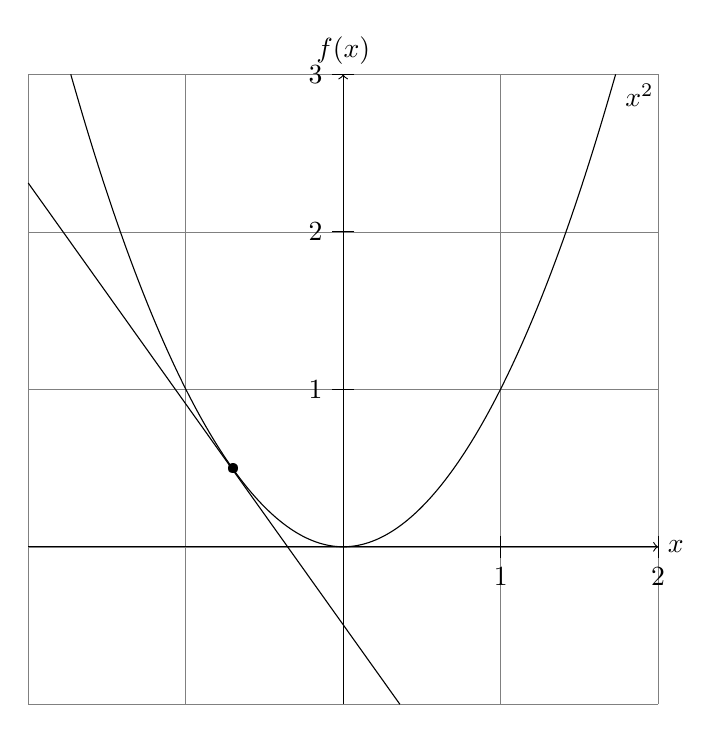
\begin{tikzpicture}[scale=2]
%  \draw[style=help lines] (0,0) grid (3.9,3.9);$
  \draw[style=help lines] (-2,-1) grid (2,3);

  \draw[->] (-2,0) -- (2,0) node[right] {$x$};
  \draw[->] (0,-1) -- (0,3) node[above] {$f(x)$};

  \foreach \x/\xtext in {1/1, 2/2}
    \draw[shift={(\x,0)}] (0pt,2pt) -- (0pt,-2pt) node[below] {$\xtext$};

  \foreach \y/\ytext in {1/1, 2/2, 3/3}
    \draw[shift={(0,\y)}] (2pt,0pt) -- (-2pt,0pt) node[left] {$\ytext$};

  \draw (-1.73,3) parabola bend (0,0) (1.73,3) node[below right] {$x^2$};
  \node at (-0.7, 0.49) {
    \textbullet
  };
  \draw (-2, 2.31) -- (0.36, -1);
\end{tikzpicture}

%% \begin{tikzpicture}[scale=2]
%%   \shade[top color=blue,bottom color=gray!50]
%%       (0,0) parabola (1.5,2.25) |- (0,0);
%%   \draw (1.05cm,2pt) node[above]
%%       {$\displaystyle\int_0^{3/2} \!\!x^2\mathrm{d}x$};

%%   \draw[style=help lines] (0,0) grid (3.9,3.9)
%%        [step=0.25cm]      (1,2) grid +(1,1);

%%   \draw[->] (-0.2,0) -- (4,0) node[right] {$x$};
%%   \draw[->] (0,-0.2) -- (0,4) node[above] {$f(x)$};

%%   \foreach \x/\xtext in {1/1, 1.5/1\frac{1}{2}, 2/2, 3/3}
%%     \draw[shift={(\x,0)}] (0pt,2pt) -- (0pt,-2pt) node[below] {$\xtext$};

%%   \foreach \y/\ytext in {1/1, 2/2, 2.25/2\frac{1}{4}, 3/3}
%%     \draw[shift={(0,\y)}] (2pt,0pt) -- (-2pt,0pt) node[left] {$\ytext$};

%%   \draw (-.5,.25) parabola bend (0,0) (2,4) node[below right] {$x^2$};
%% \end{tikzpicture}

    }
  \end{center}

  The curve needs to be \textit{smooth enough} for the gradient
  descent to work.

\end{frame}
%%%%%%%%%%%%%%%%%%%%%%%%%%%%%%%%%%%%%%%%%%%%%%%%%%%%%%%%%%%%%%%%%%%%%%

%%%%%%%%%%%%%%%%%%%%%%%%%%%%%%%%%%%%%%%%%%%%%%%%%%%%%%%%%%%%%%%%%%%%%%
\begin{frame}
  \frametitle{Gradient descent}

  \framesubtitle{Model optimization}

  \begin{center}
    \scalebox{0.5}{
      \begin{tikzpicture}[xscale = 3.5, yscale=3.5]
  \foreach \Point in { (0.418313, 0.604578), (0.196620, 0.549155),
    (0.734198, 0.683549), (0.767944, 0.691986), (0.212015, 0.553004),
    (0.866296, 0.716574), (0.741085, 0.685271), (0.091187, 0.522797),
    (0.957083, 0.739271), (0.400345, 0.600086), (0.110229, 0.527557),
    (0.628896, 0.657224), (0.079816, 0.519954), (0.585337, 0.646334),
    (0.240140, 0.560035), (0.712331, 0.678083), (0.810917, 0.702729),
    (0.262672, 0.565668), (0.690066, 0.672516), (0.871858, 0.717964),
    (0.444774, 0.611194), (0.021740, 0.505435), (0.308306, 0.577077),
    (0.055931, 0.513983), (0.343537, 0.585884), (0.007552, 0.501888),
    (0.614842, 0.653711), (0.343214, 0.585804), (0.627016, 0.656754),
    (0.951821, 0.737955) }{ 
    \node at \Point {
      \textbullet
    }; 
  }

  \draw[->] (0, 0) -- (1.2, 0) node[right] {$x$};
  \draw[->] (0, 0) -- (0, 1.2) node[above] {$y$};
  \draw (1, 0.25pt) -- (1, -0.5pt) node[anchor = north]{1};
  \draw (0.25pt, 1) -- (-0.5pt, 1) node[anchor = east]{1};
\end{tikzpicture}

    }
  \end{center}

  We have a set of points that we want to approximate with a line.

  \[
  y = ax + b
  \]

  \pause

  First we choose a loss that measures how good our predictions are.

  \[
  l(x, y, a, b) = (y - (a x + b))^{2}
  \]

  \pause

  We compute how the loss is affected by small changes of $a$ and $b$.

  \[
  \frac{\mathrm{d}l}{\mathrm{d}a} = 2 x (ax + b - y) \qquad \qquad \frac{\mathrm{d}l}{\mathrm{d}b} = 2 (ax + b - y)
  \]

  And we update $a$ and $b$ iteratively until we reach a satisfying
  result (the average loss for our data points is low enough).

%  a = -0.08 \quad b = 0.68
\end{frame}
%%%%%%%%%%%%%%%%%%%%%%%%%%%%%%%%%%%%%%%%%%%%%%%%%%%%%%%%%%%%%%%%%%%%%%

%%%%%%%%%%%%%%%%%%%%%%%%%%%%%%%%%%%%%%%%%%%%%%%%%%%%%%%%%%%%%%%%%%%%%%
\begin{frame}
  \frametitle{Gradient descent}

  \framesubtitle{Being evil}

  \vspace{-0.5cm}

  \begin{center}
    \scalebox{0.5}{
      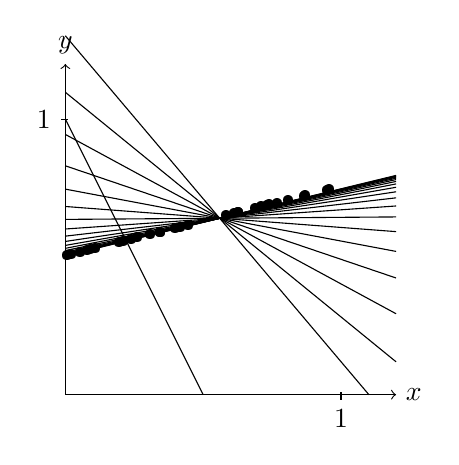
\begin{tikzpicture}[xscale = 3.5, yscale=3.5]
  \foreach \Point in { (0.418313, 0.604578), (0.196620, 0.549155),
    (0.734198, 0.683549), (0.767944, 0.691986), (0.212015, 0.553004),
    (0.866296, 0.716574), (0.741085, 0.685271), (0.091187, 0.522797),
    (0.957083, 0.739271), (0.400345, 0.600086), (0.110229, 0.527557),
    (0.628896, 0.657224), (0.079816, 0.519954), (0.585337, 0.646334),
    (0.240140, 0.560035), (0.712331, 0.678083), (0.810917, 0.702729),
    (0.262672, 0.565668), (0.690066, 0.672516), (0.871858, 0.717964),
    (0.444774, 0.611194), (0.021740, 0.505435), (0.308306, 0.577077),
    (0.055931, 0.513983), (0.343537, 0.585884), (0.007552, 0.501888),
    (0.614842, 0.653711), (0.343214, 0.585804), (0.627016, 0.656754),
    (0.951821, 0.737955) }{ 
    \node at \Point {
      \textbullet
    }; 
  }

  \draw[->] (0, 0) -- (1.2, 0) node[right] {$x$};
  \draw[->] (0, 0) -- (0, 1.2) node[above] {$y$};
  \draw (1, 0.25pt) -- (1, -0.5pt) node[anchor = north]{1};
  \draw (0.25pt, 1) -- (-0.5pt, 1) node[anchor = east]{1};
  \uncover<1>{\draw (0.000000, 1.000000) -- (0.500000, 0.000000);}
  \uncover<2>{\draw (0.000000, 1.302205) -- (1.101420, 0.000000);}
  \uncover<3>{\draw (0.000000, 1.097310) -- (1.200000, 0.119256);}
  \uncover<4>{\draw (0.000000, 0.944298) -- (1.200000, 0.293644);}
  \uncover<5>{\draw (0.000000, 0.830482) -- (1.200000, 0.423357);}
  \uncover<6>{\draw (0.000000, 0.745822) -- (1.200000, 0.519842);}
  \uncover<7>{\draw (0.000000, 0.682850) -- (1.200000, 0.591610);}
  \uncover<8>{\draw (0.000000, 0.636009) -- (1.200000, 0.644993);}
  \uncover<9>{\draw (0.000000, 0.601168) -- (1.200000, 0.684702);}
  \uncover<10>{\draw (0.000000, 0.575251) -- (1.200000, 0.714238);}
  \uncover<11>{\draw (0.000000, 0.555974) -- (1.200000, 0.736207);}
  \uncover<12>{\draw (0.000000, 0.541635) -- (1.200000, 0.752549);}
  \uncover<13>{\draw (0.000000, 0.530970) -- (1.200000, 0.764705);}
  \uncover<14>{\draw (0.000000, 0.523036) -- (1.200000, 0.773746);}
  \uncover<15>{\draw (0.000000, 0.517135) -- (1.200000, 0.780472);}
  \uncover<16>{\draw (0.000000, 0.512745) -- (1.200000, 0.785474);}
  \uncover<17>{\draw (0.000000, 0.509480) -- (1.200000, 0.789195);}
  \uncover<18>{\draw (0.000000, 0.507052) -- (1.200000, 0.791963);}
  \uncover<19>{\draw (0.000000, 0.505245) -- (1.200000, 0.794022);}
  \uncover<20>{\draw (0.000000, 0.503902) -- (1.200000, 0.795553);}
\end{tikzpicture}

    }
  \end{center}

  In our previous example, we have modified \textcolor{red}{the model}
  in order to minimize the loss.

  \[
  y = \textcolor{red}{a}x + \textcolor{red}{b}
  \]

  \pause

  Now suppose we are an attacker who wants to maximise the loss of a
  model, its \textcolor{red}{parameters} being fixed. The only thing
  we can modify is the \textcolor{blue}{inputs}.

  \[
  l(\textcolor{blue}{x}, y, a, b) = (y - (a \textcolor{blue}{x} + b))^{2}
  \]

  \pause

  In order to do this, we compute how the loss is affected by small
  changes of the input.

  \[
  \frac{\mathrm{d}l}{\mathrm{d}x} = 2 a (ax + b - y)
  \]

  We can now make \emph{imperceptible} changes to an input that will
  increase the loss value.
\end{frame}
%%%%%%%%%%%%%%%%%%%%%%%%%%%%%%%%%%%%%%%%%%%%%%%%%%%%%%%%%%%%%%%%%%%%%%

%%%%%%%%%%%%%%%%%%%%%%%%%%%%%%%%%%%%%%%%%%%%%%%%%%%%%%%%%%%%%%%%%%%%%%
\begin{frame}
  \frametitle{Neural networks}

  Everything works the same way when working with a neural network on
  an image classification task.

  \bigskip

  We also have a differentiable \textcolor{red}{loss function} (often
  \textcolor{red}{categorical cross entropy}) and
  \textcolor{blue}{inputs} (\textcolor{blue}{pixel values} in the case
  of images) that we can modify to increase the loss.
\end{frame}
%%%%%%%%%%%%%%%%%%%%%%%%%%%%%%%%%%%%%%%%%%%%%%%%%%%%%%%%%%%%%%%%%%%%%%

\section{Attack}

%%%%%%%%%%%%%%%%%%%%%%%%%%%%%%%%%%%%%%%%%%%%%%%%%%%%%%%%%%%%%%%%%%%%%%
%% \begin{frame}
%%   \frametitle{Attacks}

%%   \begin{description}
%%   \item[Random noise] Does not work
%%   \item[FGSM] Good but can be well defended by training the network
%%     with adversarial samples
%%   \item[Iterative FGSM] Higher error than FGSM for an equivalent
%%     $\varepsilon$ but less transferability. I-FGSM produces weaker
%%     black-box attacks.
%%   \item[Targeted FGSM] Aims at fooling a model into outputting a given
%%     target class.
%%   \item[RAND + FGSM] Significant improvements against adversarially
%%     trained models. RAND+FGSM transfers at lower rates than FGSM
%%     examples. Unsing RAND+FGSM to adverarially train networks does not
%%     improve their defense against RAND+FGSM.
%%   \end{description}
%% \end{frame}
%%%%%%%%%%%%%%%%%%%%%%%%%%%%%%%%%%%%%%%%%%%%%%%%%%%%%%%%%%%%%%%%%%%%%%

%%%%%%%%%%%%%%%%%%%%%%%%%%%%%%%%%%%%%%%%%%%%%%%%%%%%%%%%%%%%%%%%%%%%%%
\begin{frame}
  \frametitle{Random noise perturbation}

  \begin{center}
    \includegraphics[width = 0.7 \linewidth]{images/wait-a-minute.jpg}
  \end{center}
\end{frame}
%%%%%%%%%%%%%%%%%%%%%%%%%%%%%%%%%%%%%%%%%%%%%%%%%%%%%%%%%%%%%%%%%%%%%%

%%%%%%%%%%%%%%%%%%%%%%%%%%%%%%%%%%%%%%%%%%%%%%%%%%%%%%%%%%%%%%%%%%%%%%
\begin{frame}
  \frametitle{Random noise perturbation}

  \framesubtitle{Nope.}

  \begin{center}
    \includegraphics[width = \linewidth]{images/random_perturbation.png}
  \end{center}

\end{frame}
%%%%%%%%%%%%%%%%%%%%%%%%%%%%%%%%%%%%%%%%%%%%%%%%%%%%%%%%%%%%%%%%%%%%%%

%%%%%%%%%%%%%%%%%%%%%%%%%%%%%%%%%%%%%%%%%%%%%%%%%%%%%%%%%%%%%%%%%%%%%%
\begin{frame}
  \frametitle{Fast Gradient Sign Method [Goodfellow et al. 2015]}

  Let $x$ be the original image, $\theta$ the parameters of the model,
  $y$ the target associated with $x$ and $J(\theta, x, y)$ the loss
  function.

  \bigskip

  We compute the gradient of the loss function according to the input
  pixels.

  \[
  \nabla_{x} J(\theta, x, y)
  \]

  \bigskip

  The perturbation is the signs of these derivatives multiplied by a
  small number $\varepsilon$.

  \[
  \eta = \varepsilon \text{sign}(\nabla_{x} J(\theta, x, y))
  \]

  \bigskip

  The final adversarial sample is the sum of the original image and
  the pertubation.

  \[
  x_{adv} = x + \eta
  \]

\end{frame}
%%%%%%%%%%%%%%%%%%%%%%%%%%%%%%%%%%%%%%%%%%%%%%%%%%%%%%%%%%%%%%%%%%%%%%

%%%%%%%%%%%%%%%%%%%%%%%%%%%%%%%%%%%%%%%%%%%%%%%%%%%%%%%%%%%%%%%%%%%%%%
\begin{frame}
  \frametitle{Fast Gradient Sign Method}

  \framesubtitle{Using the \textbf{VGG16} network with imagenet
    weights}

  \begin{center}
    \begin{tikzpicture}[xscale=3.5, yscale=2]
  \node(orig) at (0, 0) {
    \includegraphics[width = 3cm]{images/FGSM_orig.png}
  };

  \node(pert) at (1, 0) {
    \includegraphics[width = 3cm]{images/FGSM_pert.png}
  };

  \node(adv) at (2, 0) {
    \includegraphics[width = 3cm]{images/FGSM_adv.png}
  };

  \node(x) at (0, 1) {
    $x$
  };

  \node(plus) at (0.5, 1) {
    +
  };

  \node(grad) at (1, 1) {
    $\varepsilon \text{sign}(\nabla_{x} L(\theta, x, y))$
  };

  \node(equal) at (1.5, 1) {
    =
  };

  \node(result) at (2, 1) {
    $x_{\text{adv}}$
  };
\end{tikzpicture}

  \end{center}
\end{frame}
%%%%%%%%%%%%%%%%%%%%%%%%%%%%%%%%%%%%%%%%%%%%%%%%%%%%%%%%%%%%%%%%%%%%%%

%%%%%%%%%%%%%%%%%%%%%%%%%%%%%%%%%%%%%%%%%%%%%%%%%%%%%%%%%%%%%%%%%%%%%%
\begin{frame}
  \frametitle{Black box attack [Papernot et al. 2016]}

  \framesubtitle{or good luck getting gradients out of your
    self-driving car}

  \begin{center}
    \includegraphics[width = 5cm]{images/cool_story_bro.jpg}
  \end{center}

\end{frame}
%%%%%%%%%%%%%%%%%%%%%%%%%%%%%%%%%%%%%%%%%%%%%%%%%%%%%%%%%%%%%%%%%%%%%%

%%%%%%%%%%%%%%%%%%%%%%%%%%%%%%%%%%%%%%%%%%%%%%%%%%%%%%%%%%%%%%%%%%%%%%
\begin{frame}
  \frametitle{Black box attack [Papernot et al. 2016]}

  \framesubtitle{Transferability of adversarial samples}

  %% If our interface with the target model is its final output, we
  %% cannot use gradients to create adversarial samples.

  We can train a new model $M'$ to solve the same classification task
  as the target model $M$.

  \pause

  \bigskip

  Once trained, we can create an adversarial sample $x_{adv}'$ for the
  $M'$ model and experiences have shown that $x_{adv}'$ will also fool
  $M$ very often.

  \pause

  \bigskip

  What if we do not have a training set for the target network?
  Well\dots{} build one using $M$ predictions.

  \pause

  \bigskip

  \textit{``After labeling 6,400 synthetic inputs to train our
    substitute (an order of magnitude smaller than the training set
    used by MetaMind) we find that their DNN misclassifies adversarial
    examples crafted with our substitute at a rate of 84.24\%''}

  \smallskip

  - Papernot et al., about their attack on the MetaMind deep neural
  network.

\end{frame}
%%%%%%%%%%%%%%%%%%%%%%%%%%%%%%%%%%%%%%%%%%%%%%%%%%%%%%%%%%%%%%%%%%%%%%

%%%%%%%%%%%%%%%%%%%%%%%%%%%%%%%%%%%%%%%%%%%%%%%%%%%%%%%%%%%%%%%%%%%%%%
\begin{frame}
  \frametitle{Adversarial examples in the physical world [Kurakin et
      al. 2017]}

  \framesubtitle{Being evil, for real}

  In real world scenarios, the target network does not take our image
  files as input. It acquires the data by the network's system
  (\textit{e.g.} a camera).

  \pause

  \medskip

  It also works, for free.

  \begin{center}
    \includegraphics[width = 7cm]{images/physical_adversarial_sample.png}
  \end{center}

%  \bigskip

  \textit{``We used images taken from a cell-phone camera as a input
    to an Inception v3 image classification neural network. We showed
    that in such a set-up, a significant fraction of adversarial
    images crafted using the original network are misclassified even
    when fed to the classifier through the camera.''}

  \smallskip

  - Kurakin et al.
\end{frame}
%%%%%%%%%%%%%%%%%%%%%%%%%%%%%%%%%%%%%%%%%%%%%%%%%%%%%%%%%%%%%%%%%%%%%%

\section{Defense}

%%%%%%%%%%%%%%%%%%%%%%%%%%%%%%%%%%%%%%%%%%%%%%%%%%%%%%%%%%%%%%%%%%%%%%
\begin{frame}
  \frametitle{Defenses}

  \begin{description}
  \item[Adversarial sample detection] We try to detect whether an
    input sample is adversarial or not before classifying it.
  \item[Regularization] Training with an adversarial objective
    function is an effective regularizer (from [explaining and
      harnessing]).
  \item[Gradient masking] The goal of gradient masking is to leave the
    decision boundaries untouched but damage the gradient used in
    white-box attacks.
  \item[Distillation and network saturation] These methods are used to
    introduce numerical instabilities in gradient computations.
  \end{description}
\end{frame}
%%%%%%%%%%%%%%%%%%%%%%%%%%%%%%%%%%%%%%%%%%%%%%%%%%%%%%%%%%%%%%%%%%%%%%

%%%%%%%%%%%%%%%%%%%%%%%%%%%%%%%%%%%%%%%%%%%%%%%%%%%%%%%%%%%%%%%%%%%%%%
\begin{frame}

  \frametitle{Defending machine learning}

  ``Most defenses against adversarial examples that have been proposed
  so far just do not work very well at all, but the ones that do work
  are not adaptive. This means it is like they are playing a game of
  whack-a-mole: they close some vulnerabilities, but leave others
  open.''

  \bigskip

  - Ian Goodfellow, Nicolas Papernot, February 2017
\end{frame}
%%%%%%%%%%%%%%%%%%%%%%%%%%%%%%%%%%%%%%%%%%%%%%%%%%%%%%%%%%%%%%%%%%%%%%

%%%%%%%%%%%%%%%%%%%%%%%%%%%%%%%%%%%%%%%%%%%%%%%%%%%%%%%%%%%%%%%%%%%%%%
\begin{frame}
  \frametitle{References}

  {\footnotesize
    \begin{enumerate}
    \item Goodfellow, I. J., Shlens, J., \& Szegedy,
      C. (2014). Explaining and harnessing adversarial
      examples. arXiv preprint arXiv:1412.6572.
    \item Papernot, N., McDaniel, P., Wu, X., Jha, S., \& Swami,
      A. (2016). Distillation as a defense to adversarial
      perturbations against deep neural networks. In Security and
      Privacy (SP), 2016 IEEE Symposium on (pp. 582-597). IEEE.
    \item Kurakin, A., Goodfellow, I., \& Bengio,
      S. (2016). Adversarial examples in the physical world. arXiv
      preprint arXiv:1607.02533.
    \item Papernot, N., McDaniel, P., Goodfellow, I., Jha, S., Celik,
      Z. B., \& Swami, A. (2016). Practical black-box attacks against
      deep learning systems using adversarial examples. arXiv preprint
      arXiv:1602.02697.
    \item Tramèr, F., Kurakin, A., Papernot, N., Boneh, D., \&
      McDaniel, P. (2017). Ensemble Adversarial Training: Attacks and
      Defenses. arXiv preprint arXiv:1705.07204.
    \end{enumerate}
  }

\end{frame}
%%%%%%%%%%%%%%%%%%%%%%%%%%%%%%%%%%%%%%%%%%%%%%%%%%%%%%%%%%%%%%%%%%%%%%

\end{document}
